% !TEX encoding = UTF-8 Unicode
\RequirePackage{fix-cm}
\documentclass[a4paper,10pt,UTF8]{paper}
%\documentclass[a4paper,10pt,UTF8]{ctexart}

\usepackage[english]{babel}
\usepackage{fancyhdr,array,lastpage,amsmath,mathtools,enumitem,graphicx,multirow,tocbibind,longtable,makecell,varwidth,titlesec,bm,booktabs,comment,minted}
\usepackage{enumitem}
\usepackage{hyperref}
\hypersetup{hidelinks}




\usepackage[left=2.54cm,right=2.54cm,top=2.54cm,bottom=2.54cm]{geometry}
\usepackage[font=footnotesize,labelfont=bf]{caption}
\usepackage{tikz,flowchart}
\usepackage{ctex}
\usepackage{xeCJK}%中文字体
\usetikzlibrary{shapes,shapes.geometric,arrows,matrix,calc}
\usetikzlibrary{circuits.logic}

% \usetikzlibrary{circuits.logic.custom}
\usetikzlibrary{circuits.logic.IEC}
\usetikzlibrary{shadows}
\usepackage{listings}
\usepackage[Q=yes]{examplep}
\usepackage{fancyhdr}
\usepackage{alphalph}
\usepackage{indentfirst}

% \setCJKsansfont{黑体}
\setmainfont{PingFang SC}
\setCJKmainfont{PingFang SC}
\setCJKsansfont{PingFang SC}
\setmonofont{Monaco}

\newenvironment{sol}
  {\par\vspace{2mm}\noindent{\bf Solution}. }

\lstset{escapeinside=``, breaklines=true, frame=none, extendedchars=false, basicstyle=\ttfamily, showstringspaces=false}


\setlength{\parindent}{2em}
\setlength{\parskip}{1.5ex plus 0.5ex minus 0.2ex}
\linespread{1.1}

\bibliographystyle{plain}

\numberwithin{equation}{section}
\numberwithin{figure}{section}

\usepackage{karnaugh}
\usepackage{circuitikz}


\setcounter{secnumdepth}{3}
\setcounter{tocdepth}{3}

\title{华东师范大学计算机科学技术系上机实验报告}

\begin{document}
\pagestyle{fancy}
\chead{\small\color{gray}华东师范大学计算机科学技术系上机实验报告}
\lhead{}
\rhead{}
\makeatletter
\def\headrule{{\if@fancyplain\let\headrulewidth\plainheadrulewidth\fi%
\color{gray}\hrule\@height 0.2pt\@width\headwidth}
  \vspace{6mm}}
\makeatother

\newcommand{\HRule}{\rule{\linewidth}{1mm}}
\newcommand{\dai}{\textbf{Dais-CMX16$^+$}}

{\center {\huge \bfseries \LARGE{华东师范大学计算机科学技术系上机实验报告}} \\ [0.8cm]
		
	\small{
		\begin{minipage}[t]{.32\linewidth}
			\textbf{课程名称:} 嵌入式系统\\
			\textbf{指导教师:} 沈建华\\
			\textbf{上机实践名称:} 汇编语言程序设计\\
			\textbf{实践编号:}实验4
		\end{minipage}
		\begin{minipage}[t]{.32\linewidth}
			\textbf{年级:}17 级\\
			\textbf{姓名:}朱桐\\
			\textbf{学号:}10175102111\\
		\end{minipage} 
		\begin{minipage}[t]{.32\linewidth}
			\textbf{上机实践成绩:} \\
			\textbf{创新实践成绩:} \\
			\textbf{上机实践日期:}2019/10/23\\
			\textbf{上机实践时间:}2 学时\\
		\end{minipage}
	}
	\HRule \\[0.5cm]
}

\definecolor{bg}{rgb}{0.95,0.95,0.95}
\newminted{asm}{bgcolor=bg}

\section{实验目的}

\begin{enumerate}
    \item 熟悉Keil中的汇编语言格式,并能熟练运用存储器访问指令、逻辑操作指令、移位操作指令(LSL、LSR、ASR、ROR、RRX等),熟悉其功能及用法
    \item 熟练掌握基本汇编程序的程序语法及设计格式;
\end{enumerate}

\section{实验设备}

软件开发系统Keil5;

\section{实验内容}

\begin{itemize}
  \item 学习并掌握简单的ARM汇编指令,熟悉其功能及用法,根据题目编写ARM汇编程序;
  \item 了解奇偶校验码原理及其基本计算方法,并用汇编语言实现;
  \item 了解海明码原理及其基本计算方法,并用汇编语言实现;
\end{itemize}

\section{实验原理}

\subsection{奇偶校验码原理}

在原编码上加一个校验位,它的码距等于2,可以检测出一位错误(或奇数位错误),但不能确定出错的位置,也不能够检测偶数位错误,增加的冗余位称为奇偶校验位。

由若干位有效信息和一个二进制位(校验位)组成校验码。校验位的取值(0或1)将使整个校验码中”1”的个数为奇数或偶数,所以有两种可供选择的校验规律。

奇校验码:整个校验码(有效信息位和校验位)中''1''的个数为奇数。

偶校验码:整个校验码(有效信息位和校验位)中''1''的个数为偶数。

举例:

100 1101 (原编码,设最低位为校验位)

1001 1011(奇校验码)

1001 1010(偶校验码)

\subsection{海明码原理}

接收端对这r个偶关系进行校验,即将每个冗余位和与它相关联的信息位进行异或运算,相异或地结果称为校正因子。

如果没有错的话,这r个校正因子都为0;如果有一个错则校正因子不会全为0,根据校正因子的不同取值,可以知道错误发生在码字的哪一个位置上。

\subsubsection{海明码的构造及校验方法}


\begin{itemize}
  \item 根据关系式 $2^r \ge k+r+1$,计算冗余位的位数;
  \item 确定信息位与冗余位的位置关系,2i(i=0,1…r)的位置上放冗余位ri,其余位置上Ij(j=1,..k);
  \item 找出冗余位与信息位的校验关系;
  \item 根据校验关系来确定冗余位。
\end{itemize}

教材给出的 PPT 并没有给出如何构造校验关系的方法,而是针对习题直接给出了校验关系式。这里本着对海明码的好奇,结合网上资料我实现了自动寻找海明码的功能(这样完全摆脱了身边大多数人写的硬编码的弊端,如果更改位数将几乎不用改动代码,而这些人写的代码只能对一种要求实现功能,否则要几乎重写代码)

海明码的中心思想是将 $2^n$ 位置用来作为冗余码,然后假定只有一个位置出错,用冗余码去确定哪个位置出错。换言之,我们需要用 $2^n$ 这些位置来表示唯一的位置。可这不是很简单嘛?使用二进制表达任何一个数,二进制位模式为 1,我们就让对应的冗余码去包含这个位置上的数据。那么如果只有这个数据出错,对应二进制位置上的冗余码就恰好由 0 变为 1,正好就出现了我们想要的——找到出错位置的唯一位置

接下来将描述算法的过程,我个人觉得先看算法的描述对算法的理解有帮助,以存放 4 位数 1101 为例,假设最后的海明码为 $\overline{H_1H_2...H_k}$,原码位 $\overline{l_4l_3l_2l_1}$


\begin{enumerate}
  \item 冗余位个数为3,分别存放在 $H_1,H_2,H_4$
  \item 剩下的位则存放在 $H_3,H_5,H_6,H_7$
  \item 3 的位模式 $0011$,可以理解为 $H_{1+2}$
  \item 5 对应可以理解为 $H_{4+1}$
  \item 6 对应 $H_{4+2}$
  \item 7 对应 $H_{4+2+1}$
  \item 涉及 $H_1$ 的有 $H_3,H_5,H_7$,那么 $r_0 = H_3 \oplus H_5 \oplus H_7 = l_1 \oplus l_2 \oplus l_4$
  \item 同理 $r_1 = l_4 \oplus l_3 \oplus l_1$
  \item $r_2 = l_4 \oplus l_3 \oplus l_2$
\end{enumerate}

推广来说,我们寻找的关系就是用冗余位的下标在加法下凑出信息位的下标,然后对应找出每个冗余位涉及的信息位,这些信息位的异或和就是冗余位

\section{实验步骤}

\subsection{联系1}

相对实验2来说十分简单的练习,只要不断循环右移,获取二进制末尾的一项,然后统计 1 出现的次数就行了

\begin{asmcode}
  AREA Reset,DATA,READONLY
  DCD 0X12345678
  DCD   Reset_Handler
  AREA CODE_SEGMET,CODE,READONLY
Reset_Handler  proc
  export Reset_Handler    [weak]
    ;MOV R0,#0xA     ;用例1输入值0xA,结果0x15
    ;MOV R0,#0xBA     ;用例2输入值0xAB,结果0x174
    ;MOV R0,#0xCBA   ;用例3输入值0xABC,结果0x1974
    MOV R0,#0x7654  ;用例4输入值0x7654,结果0xECA9
    MOV R1,R0       ;R1存储结果
    MOV R2,#0       ;R2存储1的个数
    MOV R3,#0       ;R3作为临时寄存器,最多只能使用R0、R1、R2、R3及xPSR寄存器
    ;//---------------请在以下空白区域内编写代码------------//

LOOPI
  AND R3,R0,#1
  ADD R2,R2,R3
  LSRS R0,R0,#1
  BGT LOOPI
  AND R3,R2,#1
  EOR R1,R3,#1
    ;//---------------请在以上空白区域内编写代码------------//
    ;最终结果存入R1
    NOP         ;请直接跳转至此
  ENDP
  END
\end{asmcode}
\subsection{实验2}

主要的精力花费在了完成实验2的代码

首先是不断循环右移,判断给定的数据有多少位 $k$, 然后完成不等式 $2^r+r \le k+1$ 的计算,确定在原代码有 $k$ 位的情况下,冗余位有 $r$ 位,方法是不断使 $r \leftarrow r+1$ 然后判断

\begin{itemize}
  \item R0: 输入的数
  \item R1: 临时变量
  \item R2: 信息位个数 $k$
  \item R3: 冗余位个数 $r$
\end{itemize}

\begin{asmcode}
NUMBER_BIT
  ADD R2,R2,#1
    LSRS R1,R1,#1
    BGT NUMBER_BIT
  MOV R3,#0 
  ; R3 = r, R2 = k, 2^r-r-1 >= K, R4 for tmp, 
  ; this loop is to determine r
LOOPRK
  ADD R3,R3,#1
  MOV R4, #1
  LSL R4, R4, R3
  SUB R4,R4,R3
  SUB R4,R4,#1
  SUBS R4,R4,R2
  BLT LOOPRK
\end{asmcode}


然后接着就是计算海明码。这里大概的思路是,每次循环 $R4=2^x,R5=R5+1$,当 $R4=R5$ 时,说明当前应该填的是冗余码并且更新 $R4=R4 \times 2$,否则填入信息码

\begin{itemize}
  \item R4: 冗余码位置 $2^x$
  \item R5: 当前要填的海明码位置
  \item R6: 当前要填进去的信息位个数
\end{itemize}

\begin{asmcode}
  ; dump k bit int to k+r bit Hamming Code in R1, R7,R8,R9,R10 for tmp
  MOV R1,#0
  MOV R4, #1 ;R4 stands for the next 2^n
  MOV R5, #1 ;R5 stands for the current bit in hamming code
  MOV R6, #0 ;R6 stands for the current bit in original int
DUMP
  CMP R5,R4
  LSLEQ R4,R4,#1 ; should prepare for the next parity code,
  ; instead of setting information bit
  MOV R7,#1
  LSL R7,R7,R6 ; R7 = 2^{R6} & R0, get the R6-th bit in original int
  ANDS R7,R7,R0
  MOV R7,#0
  MOVNE R7,#1 ; R6 = 2^{R5-1}, prepare to set the R5-th bit 
  ;in hamming code
  SUB R5,R5,#1
  LSL R7,R7,R5
  ADD R5,R5,#1
  CMP R4,R5,LSL #1
  BEQ CONT
  EOR R1,R1,R7 ; copy the $R6-th bit in original int to the $R5-th bit in hamming-code
  ADD R6,R6,#1
  CBZ R7,CONT
  MOV R8,R5
  MOV R10,#0
\end{asmcode}

之后如果是信息码且该位为 1,我们就要反转合适的冗余码。这里又需要进行二进制转换

\begin{asmcode}
LOOP
  ANDS R7,R8,#1
  MOV R9,#0
  MOVNE R9,#1
  LSLS R9,R9,R10
  MOV R7,#1
  SUBNE R9,R9,#1
  LSLNE R9,R7,R9
  EOR R1,R1,R9
  
  LSRS R8,R8,#1
  ADD R10,R10,#1
  BNE LOOP
\end{asmcode}

最后是进行 $R5=R5+1$ 并且继续循环

\begin{asmcode}
CONT
  ADD R5,R5,#1
  CMP R6,R2
  BLT DUMP
\end{asmcode}

完整的计算海明码如下:

\begin{asmcode}
  ; dump k bit int to k+r bit Hamming Code in R1, R7,R8,R9,R10 for tmp
  MOV R1,#0
  MOV R4, #1 ;R4 stands for the next 2^n
  MOV R5, #1 ;R5 stands for the current bit in hamming code
  MOV R6, #0 ;R5 stands for the current bit in original int
DUMP
  CMP R5,R4
  LSLEQ R4,R4,#1 ; should prepare for the next parity code, 
  ;instead of setting information bit
  MOV R7,#1
  LSL R7,R7,R6 ; R7 = 2^{R6} & R0, get the R6-th bit in original int
  ANDS R7,R7,R0
  MOV R7,#0
  MOVNE R7,#1 ; R6 = 2^{R5-1}, prepare to set the R5-th bit 
  ;in hamming code
  SUB R5,R5,#1
  LSL R7,R7,R5
  ADD R5,R5,#1
  CMP R4,R5,LSL #1
  BEQ CONT
  EOR R1,R1,R7 ; copy the $R6-th bit in original int to the 
  ;$R5-th bit in hamming-code
  ADD R6,R6,#1
  CBZ R7,CONT
  MOV R8,R5
  MOV R10,#0
LOOP
  ANDS R7,R8,#1
  MOV R9,#0
  MOVNE R9,#1
  LSLS R9,R9,R10
  MOV R7,#1
  SUBNE R9,R9,#1
  LSLNE R9,R7,R9
  EOR R1,R1,R9
  
  LSRS R8,R8,#1
  ADD R10,R10,#1
  BNE LOOP
CONT
  ADD R5,R5,#1
  CMP R6,R2
  BLT DUMP
\end{asmcode}

之后我们改变 $R0$ 寄存器的数字,重新计算海明码,这里我们把冗余位和老的海明码一起备份在 $R11$


\begin{asmcode}
  MOV R11,R1 ; backup the parity code
  MOV R8,#1
  EOR R0,R8,LSL #3; change the 3-th bit of R0
  
  ; same again, calc the parity code for new hamming code
  ; dump k bit int to k+r bit Hamming Code in R1, R7,R8,R9,R10 for tmp
  MOV R1,#0
  MOV R4, #1 ;R4 stands for the next 2^n
  MOV R5, #1 ;R5 stands for the current bit in hamming code
  MOV R6, #0 ;R5 stands for the current bit in original int
DUMP2
  CMP R5,R4
  LSLEQ R4,R4,#1 ; should
  ......
\end{asmcode}

然后通过比较冗余位,计算出是哪个位置出错

\begin{itemize}
  \item R5 正在比较海明码的位置
  \item R6,R9 临时变量
  \item R7,R8 两个海明码的冗余位数值提取
\end{itemize}

\begin{asmcode}
FLOOP
  MOV R6,#1
  LSL R6,R6,R5
  MOV R9,#1
  SUB R6,R6,#1
  LSL R6,R9,R6
  AND R7,R1,R6
  AND R8,R11,R6
  EORS R6,R7,R8
  MOV R9,#1
  LSL R9,R9,R5
  ADDNE R4,R4,R9
  
  ADD R5,R5,#1
  CMP R5,R3
  BLT FLOOP
\end{asmcode}

最后,从海明码变回原数,存回 R0, 此时 R0 将变回初始的值,方法和转换海明码部分类似

\begin{asmcode}
  DUMPR ; convert hamming code to original code in R0
  CMP R5,R4
  LSLEQ R4,R4,#1 ; parity code
  BEQ CONTR
  MOV R7,#1
  SUB R5,R5,#1
  LSL R7,R7,R5
  ADD R5,R5,#1
  ANDS R7,R7,R1
  MOV R8,#0
  MOVNE R8,#1
  LSL R8,R8,R6
  EOR R0,R0,R8
  ADD R6,R6,#1
CONTR
  ADD R5,R5,#1
  CMP R6,R2
  BLT DUMPR
; now R0 is restored!
\end{asmcode}

总之,最后的代码又丑又长,不过勉强完成了功能。写完之后才发现有些地方完全可以写得更加优雅


\section{调试过程、结果与分析}

这个程序只要满足海明码位数小于31位(通用寄存器能存的下),都可以完成功能。我们令输入数据为, 0xD, 0xAB, 0xABC,这里给出输入为 0xAB (按照实验要求)的运行截图。实际上,对于三种输入都能得出正确的结果。

\subsection{输入为 0xAB}


计算位数,相关寄存器 R2,R3,如图 \ref{fig:5}

\begin{figure}[h]
  \centering
  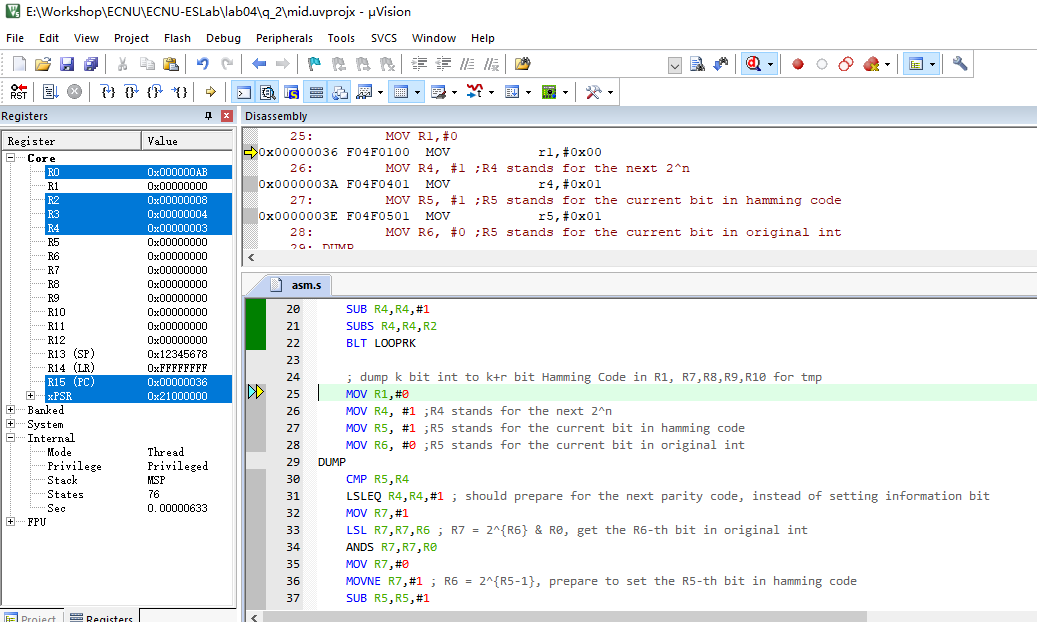
\includegraphics[width=0.9\linewidth]{1.PNG}
  \caption{计算位数}
  \label{fig:5}
\end{figure}

计算海明码并且更改R0,相关寄存器 R0,R1,如图 \ref{fig:6}

\begin{figure}[h]
  \centering
  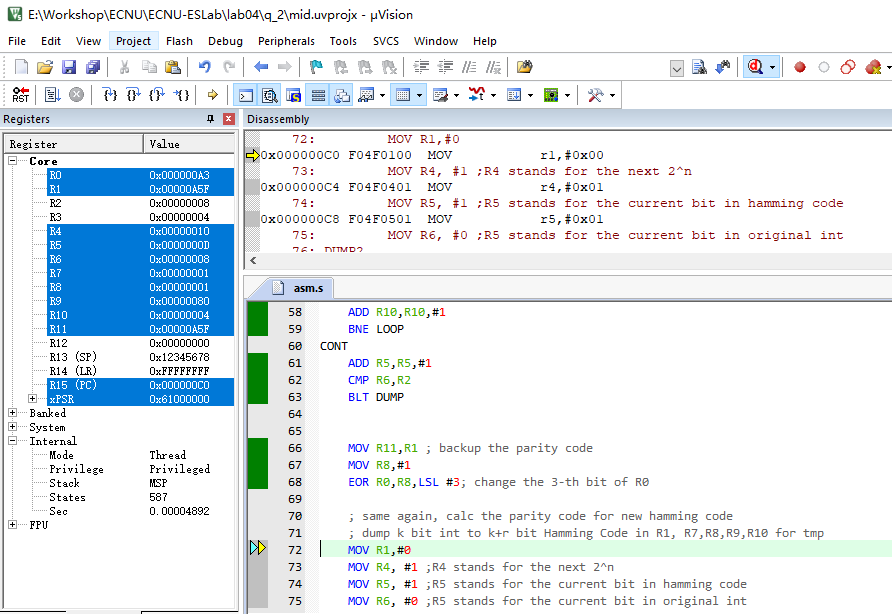
\includegraphics[width=0.9\linewidth]{2.PNG}
  \caption{计算冗余码更改}
  \label{fig:6}
\end{figure}

计算海明码的第七位,也就是数据的第四位(从1开始计数)出现错误,如图 \ref{fig:7}


\begin{figure}[h]
  \centering
  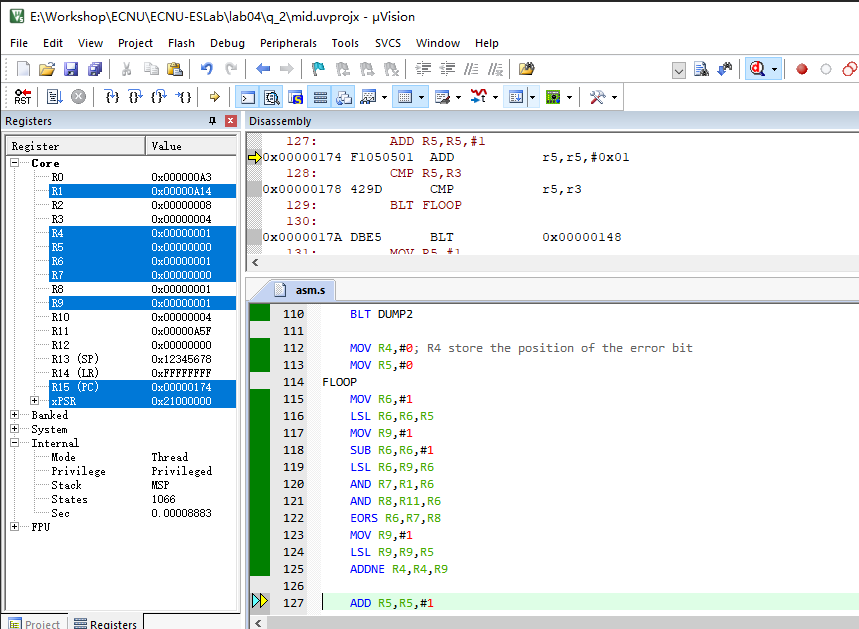
\includegraphics[width=0.9\linewidth]{3.png}
  \caption{计算海明码的第七位出错}
  \label{fig:7}
\end{figure}

将海明码转换回原编码,并且纠错,得到最开始的答案,如图 \ref{fig:8}


\begin{figure}[h]
  \centering
  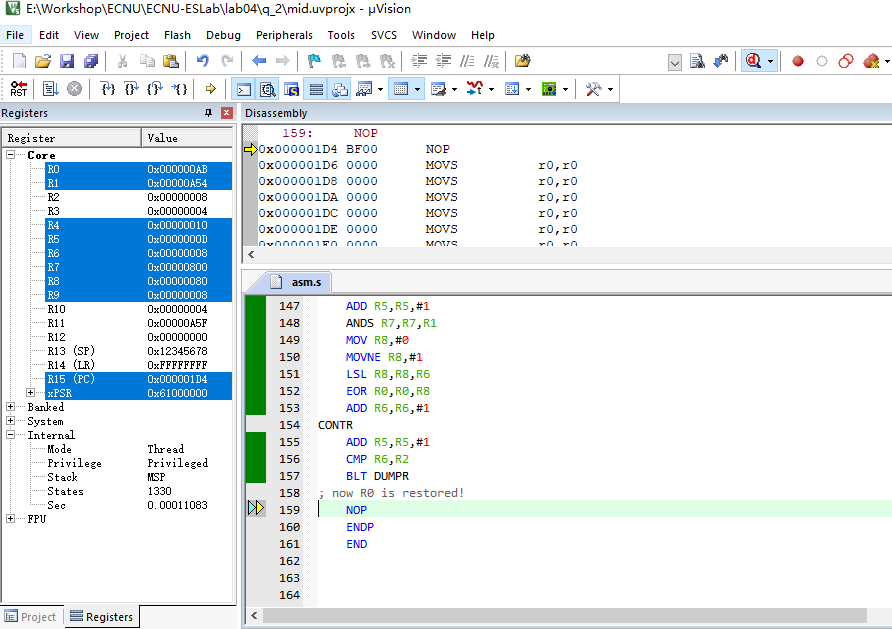
\includegraphics[width=0.9\linewidth]{4.png}
  \caption{恢复原来 R0}
  \label{fig:8}
\end{figure}

\section{总结}

第二个练习的代码最后写得又丑又长,其实主要还是因为没有提前规划好设计模式,仍有一些可以改进的空间

\begin{enumerate}
  \item 设计二进制转换,比如循环 $x$ 要获取 $2^x$,可以令 $R0=1,R0=R0+R0$ 而不是再 $R0=0,R0=R0+1$ 然后在用左移获取 $2^x$ 的值
  \item 有两次计算海明码的过程,这个过程用函数调用实现显然会更加优雅
  \item 临时寄存器大乱炖,这个可以通过提前规划解决
  \item 部分功能有更少的代码可以实现
  \item ...
\end{enumerate}



\section{附件}

完整代码如下

第一个练习

\begin{asmcode}
  AREA Reset,DATA,READONLY
  DCD 0X12345678
  DCD   Reset_Handler
  AREA CODE_SEGMET,CODE,READONLY
Reset_Handler  proc
  export Reset_Handler    [weak]
    ;MOV R0,#0xA     ;用例1输入值0xA,结果0x15
    ;MOV R0,#0xBA     ;用例2输入值0xAB,结果0x174
    ;MOV R0,#0xCBA   ;用例3输入值0xABC,结果0x1974
    MOV R0,#0x7654  ;用例4输入值0x7654,结果0xECA9
    MOV R1,R0       ;R1存储结果
    MOV R2,#0       ;R2存储1的个数
    MOV R3,#0       ;R3作为临时寄存器,最多只能使用R0、R1、R2、R3及xPSR寄存器
    ;//---------------请在以下空白区域内编写代码------------//

LOOPI
  AND R3,R0,#1
  ADD R2,R2,R3
  LSRS R0,R0,#1
  BGT LOOPI
  AND R3,R2,#1
  EOR R1,R3,#1
    ;//---------------请在以上空白区域内编写代码------------//
    ;最终结果存入R1
    NOP         ;请直接跳转至此
  ENDP
  END
\end{asmcode}

第二个练习

\begin{asmcode}
	AREA Reset,DATA,READONLY
	DCD 0X12345678
	DCD   Reset_Handler
	AREA CODE_SEGMET,CODE,READONLY
Reset_Handler  proc
	export Reset_Handler    [weak]
    MOV R0,0xABC ; input data, you can input whatever int you want
    MOV R1,R0
    MOV R2,#0 ; store the number of bit of the input number, this loop is to determine k
NUMBER_BIT
	ADD R2,R2,#1
    LSRS R1,R1,#1
    BGT NUMBER_BIT
	MOV R3,#0 ; R3 = r, R2 = k, 2^r-r-1 >= K, R4 for tmp, this loop is to determine r
LOOPRK
	ADD R3,R3,#1
	MOV R4, #1
	LSL R4, R4, R3
	SUB R4,R4,R3
	SUB R4,R4,#1
	SUBS R4,R4,R2
	BLT LOOPRK

	; dump k bit int to k+r bit Hamming Code in R1, R7,R8,R9,R10 for tmp
	MOV R1,#0
	MOV R4, #1 ;R4 stands for the next 2^n
	MOV R5, #1 ;R5 stands for the current bit in hamming code
	MOV R6, #0 ;R5 stands for the current bit in original int
DUMP
	CMP R5,R4
	LSLEQ R4,R4,#1 ; should prepare for the next parity code, instead of setting information bit
	MOV R7,#1
	LSL R7,R7,R6 ; R7 = 2^{R6} & R0, get the R6-th bit in original int
	ANDS R7,R7,R0
	MOV R7,#0
	MOVNE R7,#1 ; R6 = 2^{R5-1}, prepare to set the R5-th bit in hamming code
	SUB R5,R5,#1
	LSL R7,R7,R5
	ADD R5,R5,#1
	CMP R4,R5,LSL #1
	BEQ CONT
	EOR R1,R1,R7 ; copy the $R6-th bit in original int to the $R5-th bit in hamming-code
	ADD R6,R6,#1
	CBZ R7,CONT
	MOV R8,R5
	MOV R10,#0
LOOP
	ANDS R7,R8,#1
	MOV R9,#0
	MOVNE R9,#1
	LSLS R9,R9,R10
	MOV R7,#1
	SUBNE R9,R9,#1
	LSLNE R9,R7,R9
	EOR R1,R1,R9
	
	LSRS R8,R8,#1
	ADD R10,R10,#1
	BNE LOOP
CONT
	ADD R5,R5,#1
	CMP R6,R2
	BLT DUMP
	
	
	MOV R11,R1 ; backup the parity code
	MOV R8,#1
	EOR R0,R8,LSL #3; change the 3-th bit of R0
	
	; same again, calc the parity code for new hamming code
	; dump k bit int to k+r bit Hamming Code in R1, R7,R8,R9,R10 for tmp
	MOV R1,#0
	MOV R4, #1 ;R4 stands for the next 2^n
	MOV R5, #1 ;R5 stands for the current bit in hamming code
	MOV R6, #0 ;R5 stands for the current bit in original int
DUMP2
	CMP R5,R4
	LSLEQ R4,R4,#1 ; should prepare for the next parity code, instead of setting information bit
	MOV R7,#1
	LSL R7,R7,R6 ; R7 = 2^{R6} & R0, get the R6-th bit in original int
	ANDS R7,R7,R0
	MOV R7,#0
	MOVNE R7,#1 ; R6 = 2^{R5-1}, prepare to set the R5-th bit in hamming code
	SUB R5,R5,#1
	LSL R7,R7,R5
	ADD R5,R5,#1
	CMP R4,R5,LSL #1
	BEQ CONT2
	EOR R1,R1,R7 ; copy the $R6-th bit in original int to the $R5-th bit in hamming-code
	ADD R6,R6,#1
	CBZ R7,CONT2
	MOV R8,R5
	MOV R10,#0
LOOP2
	ANDS R7,R8,#1
	MOV R9,#0
	MOVNE R9,#1
	LSLS R9,R9,R10
	MOV R7,#1
	SUBNE R9,R9,#1
	LSLNE R9,R7,R9
	EOR R1,R1,R9
	
	LSRS R8,R8,#1
	ADD R10,R10,#1
	BNE LOOP2
CONT2
	ADD R5,R5,#1
	CMP R6,R2
	BLT DUMP2

	MOV R4,#0; R4 store the position of the error bit
	MOV R5,#0
FLOOP
	MOV R6,#1
	LSL R6,R6,R5
	MOV R9,#1
	SUB R6,R6,#1
	LSL R6,R9,R6
	AND R7,R1,R6
	AND R8,R11,R6
	EORS R6,R7,R8
	MOV R9,#1
	LSL R9,R9,R5
	ADDNE R4,R4,R9
	
	ADD R5,R5,#1
	CMP R5,R3
	BLT FLOOP

	MOV R5,#1
	SUB R4,R4,#1
	LSL R4,R5,R4
	EOR R1,R1,R4 ; now the bit on the hamming code should be corrected
	
	MOV R0,#0
	MOV R4, #1 ;R4 stands for the next 2^n
	MOV R5, #1 ;R5 stands for the current bit in hamming code
	MOV R6, #0 ;R5 stands for the current bit in original int
DUMPR ; convert hamming code to original code in R0
	CMP R5,R4
	LSLEQ R4,R4,#1 ; parity code
	BEQ CONTR
	MOV R7,#1
	SUB R5,R5,#1
	LSL R7,R7,R5
	ADD R5,R5,#1
	ANDS R7,R7,R1
	MOV R8,#0
	MOVNE R8,#1
	LSL R8,R8,R6
	EOR R0,R0,R8
	ADD R6,R6,#1
CONTR
	ADD R5,R5,#1
	CMP R6,R2
	BLT DUMPR
; now R0 is restored!
    NOP
	ENDP
	END  
\end{asmcode}

\end{document}
